% !TeX spellcheck = de_DE

\chapter{Kalibrierung}
\label{chap:calibration}

Nachdem im vorherigen Kapitel auf die Methode der Dilatation zur Verbesserung des erstellten Tiefenbildes eingegangen wurde, wird in diesem Kapitel der Vorgang der Kalibrierung beschrieben.

\section{Ziele der Kalibrierung}
Das Ziel bei unserer Kalibrierung ist es die Bilder zweier verschiedener Kameras aufeinander anzupassen, sodass in beiden Kameras das gleiche Bild angezeigt wird.

\begin{figure}[h]
	\centering
	\begin{subfigure}[t]{0.45\textwidth}
		\centering
		\ifthenelse{\boolean{jpg}}{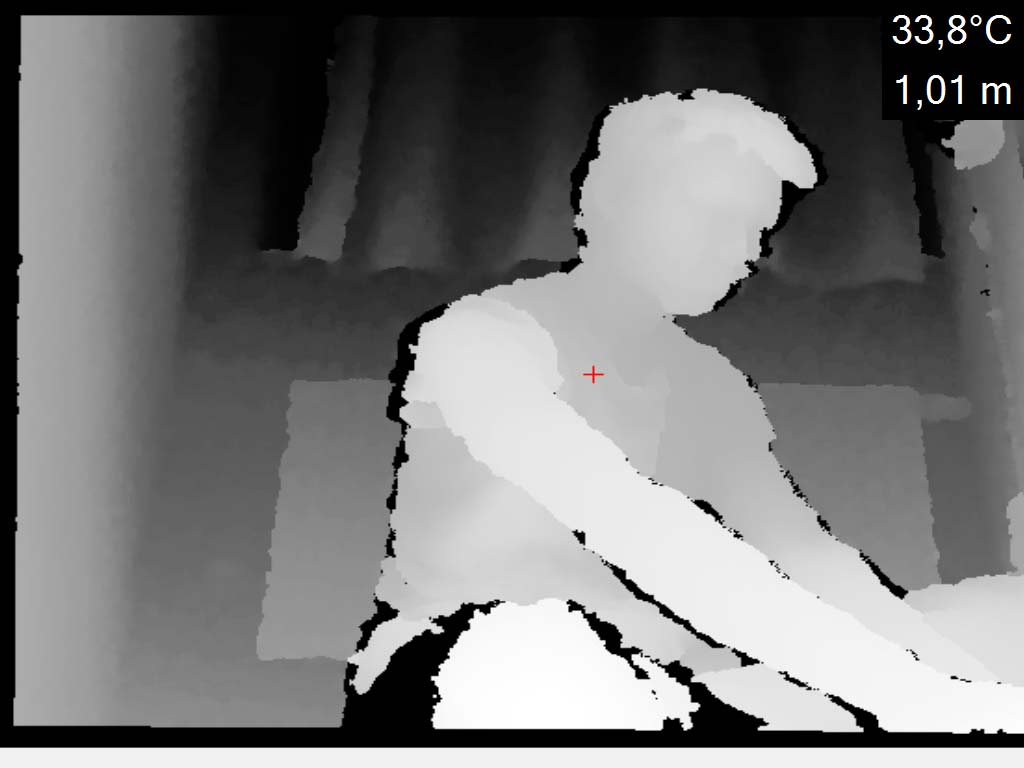
\includegraphics[width=\textwidth]{Kalibrierung/pre_depth.jpg}}{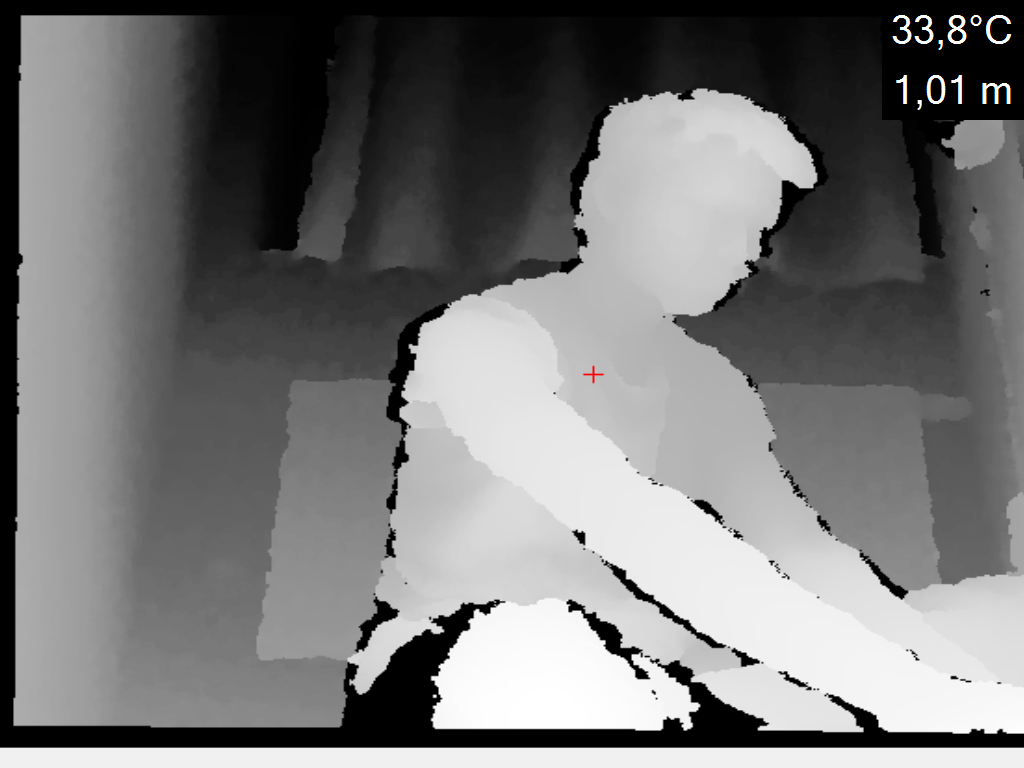
\includegraphics[width=\textwidth]{Kalibrierung/pre_depth.png}}
		\caption{Tiefenbild}
		\label{fig:calib_pre_deepth}
	\end{subfigure}
	~
	\begin{subfigure}[t]{0.45\textwidth}
		\centering
		\ifthenelse{\boolean{jpg}}{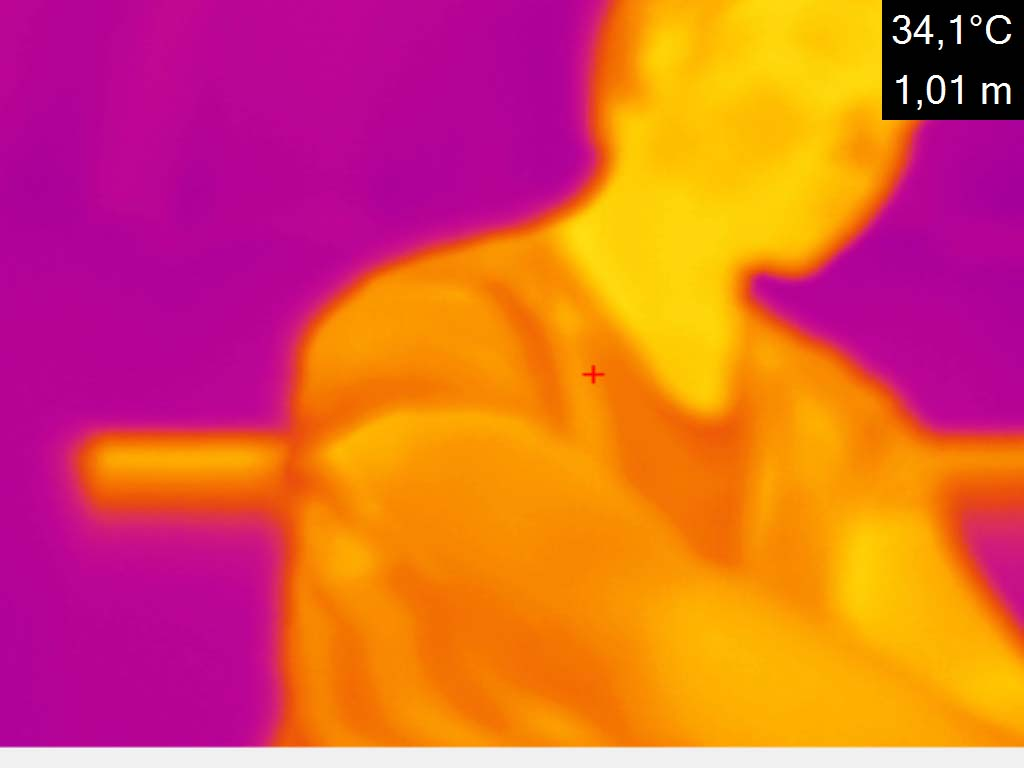
\includegraphics[width=\textwidth]{Kalibrierung/pre_heat.jpg}}{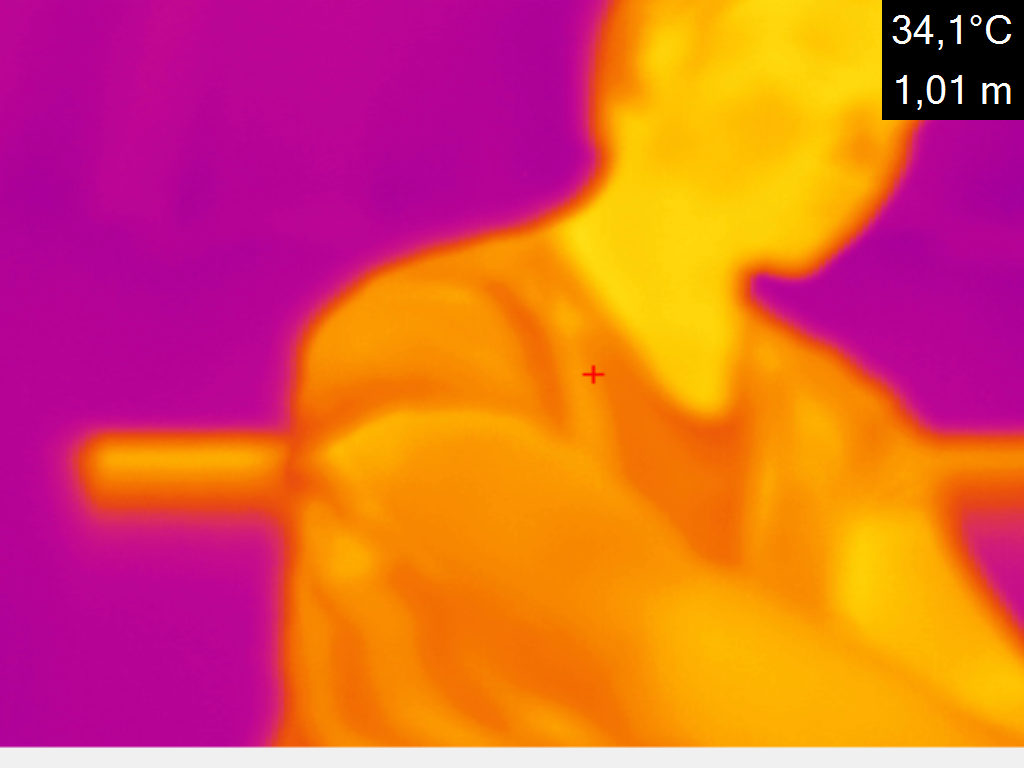
\includegraphics[width=\textwidth]{Kalibrierung/pre_heat.png}}
		\caption{Wärmebild}
		\label{fig:calib_pre_heat}
	\end{subfigure}
	\caption{Kamerabilder vor der Kalibrierung}
	\label{fig:calib_pre}
\end{figure}

\begin{figure}[h]
	\centering
	\begin{subfigure}[t]{0.45\textwidth}
		\centering
		\ifthenelse{\boolean{jpg}}{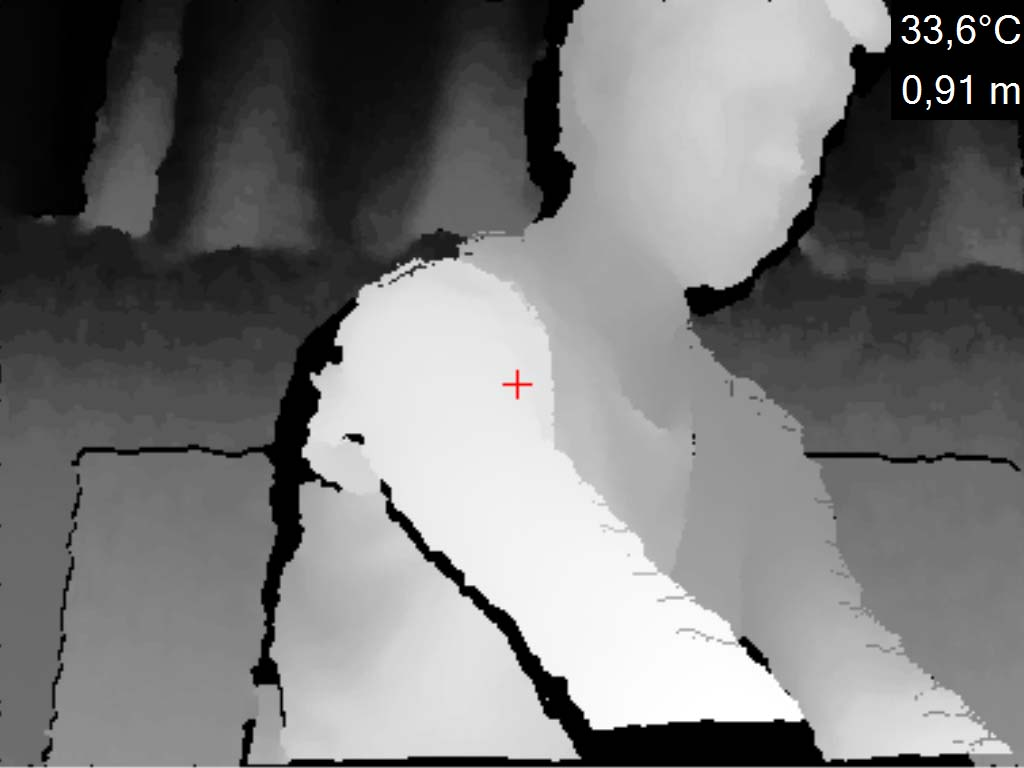
\includegraphics[width=\textwidth]{Kalibrierung/post_depth.jpg}}{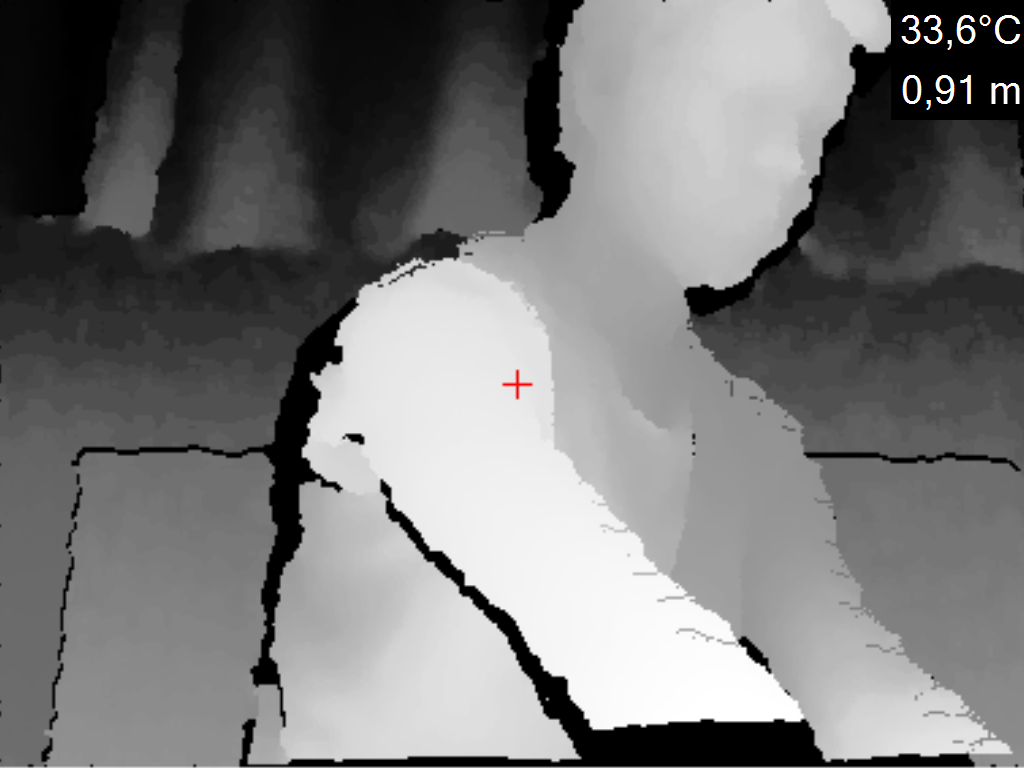
\includegraphics[width=\textwidth]{Kalibrierung/post_depth.png}}
		\caption{Tiefenbild}
		\label{fig:calib_post_deepth}
	\end{subfigure}
	~
	\begin{subfigure}[t]{0.45\textwidth}
		\centering
		\ifthenelse{\boolean{jpg}}{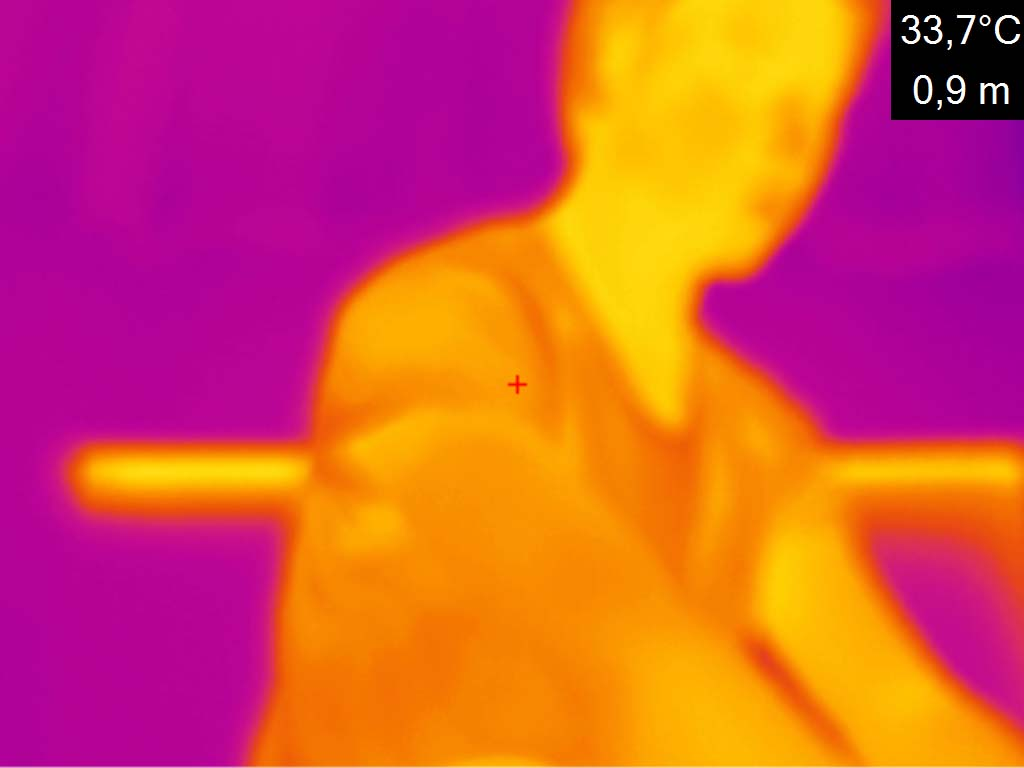
\includegraphics[width=\textwidth]{Kalibrierung/post_heat.jpg}}{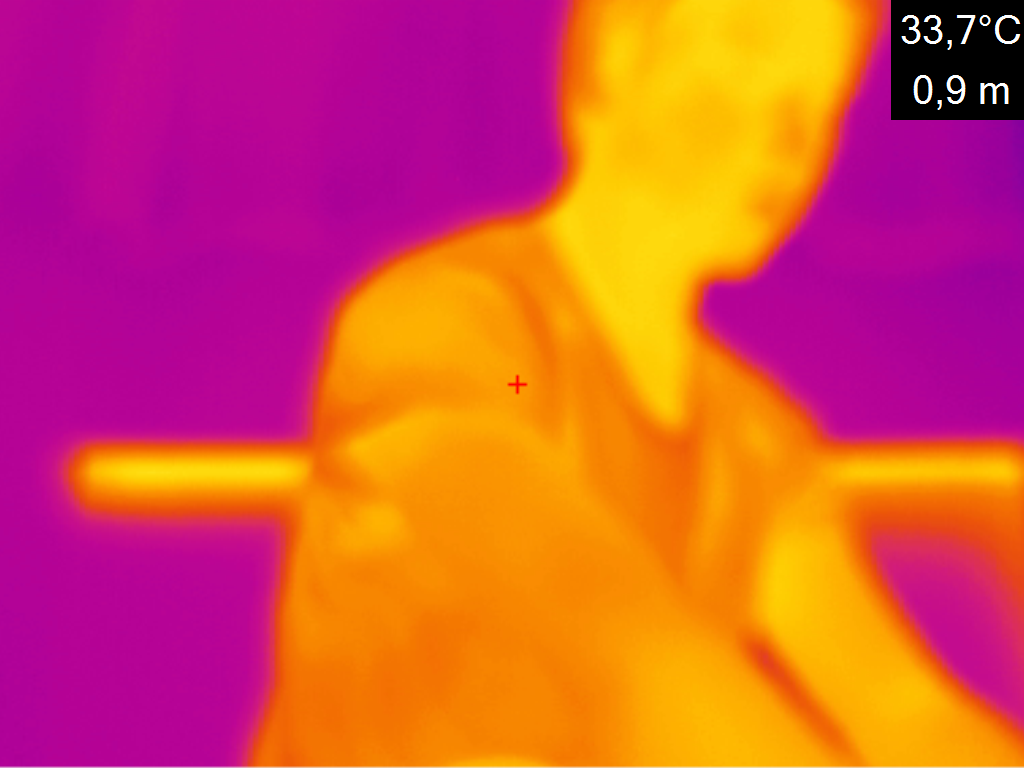
\includegraphics[width=\textwidth]{Kalibrierung/post_heat.png}}
		\caption{Wärmebild}
		\label{fig:calib_post_heat}
	\end{subfigure}
	\caption{Kamerabilder nach der Kalibrierung}
	\label{fig:calib_ost}
\end{figure}

Dafür werden benötigt:
\begin{description}
	\item[intrinsischer Kameraparameter] Bestehend aus:
	\begin{itemize}
		\item Fokallänge (focal length) 
		\item Bildmittelpunkt (principal point)
	\end{itemize}
	\item[extrinsischer Kameraparameter] Bestehend aus:
	\begin{itemize}
		\item Rotationsmatrix
		\item Translationsmatrix
	\end{itemize}
\end{description}

\section{Berechnung der intrinsischen und extrinsischen Kameraparameter}
Diese intrinsischen und extrinsischen Kameraparameter wurden für uns in MATLAB mithilfe der Computer Vision Toolbox berechnet.
\begin{figure}[h]
	\centering
	\ifthenelse{\boolean{jpg}}{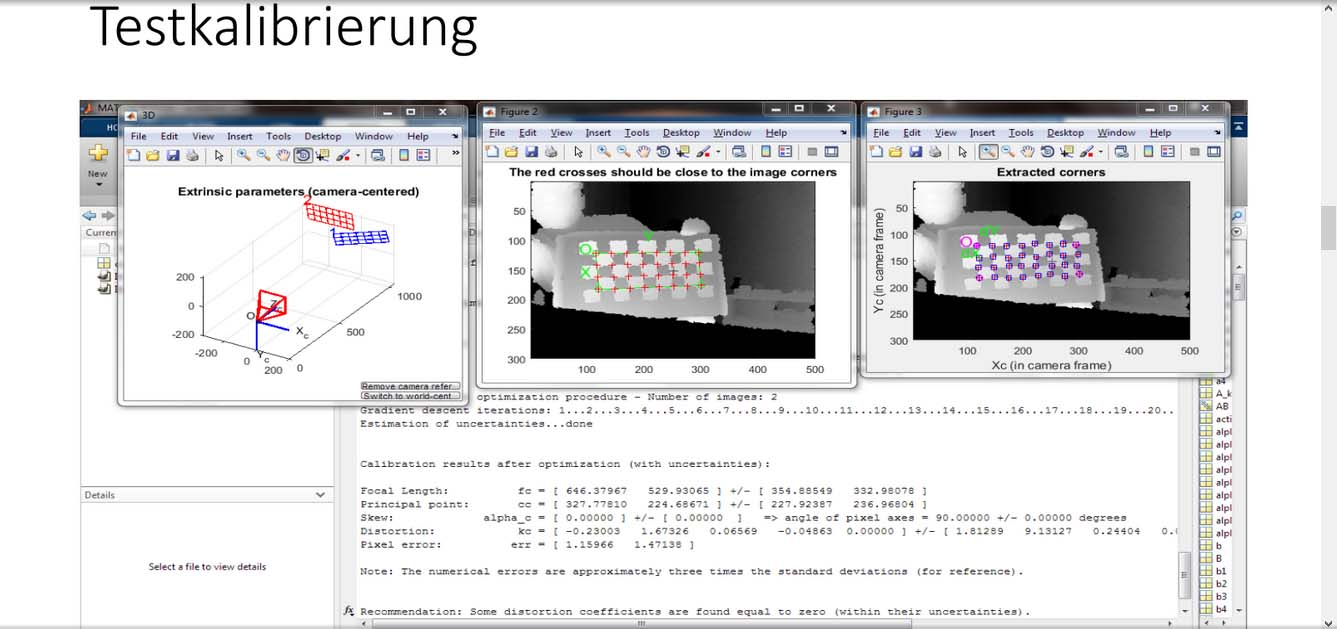
\includegraphics[width=\textwidth]{Kalibrierung/MatLab.jpg}}{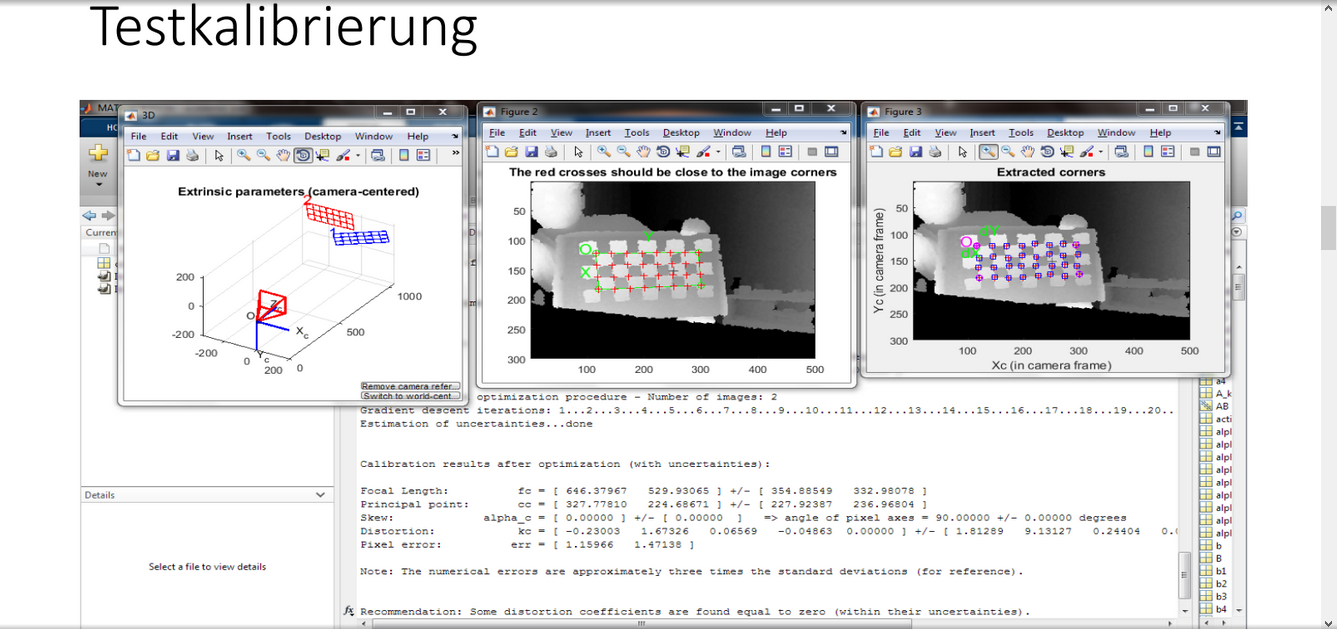
\includegraphics[width=\textwidth]{Kalibrierung/MatLab.png}}
	\caption{Testkalibrierung mit MATLAB}
	\label{fig:calib_matlab}
\end{figure}

\subsection{Vorgehen}
Es werden von den beiden zu kalibrierenden Sensoren Bilder von einem Schachbrett gemacht.
Dabei sollten diese Bilder möglichst aus verschiedene Positionen und und Winkeln erstellt werden.
Mithilfe von MATLAB kann dann durch diese Bilder die intrischen Kameraparameter und extrinsischen Kameraparameter, welche die Position zwischen den beiden Sensoren beschreibt berechnet werden.
\begin{figure}[h]
	\centering
	\ifthenelse{\boolean{jpg}}{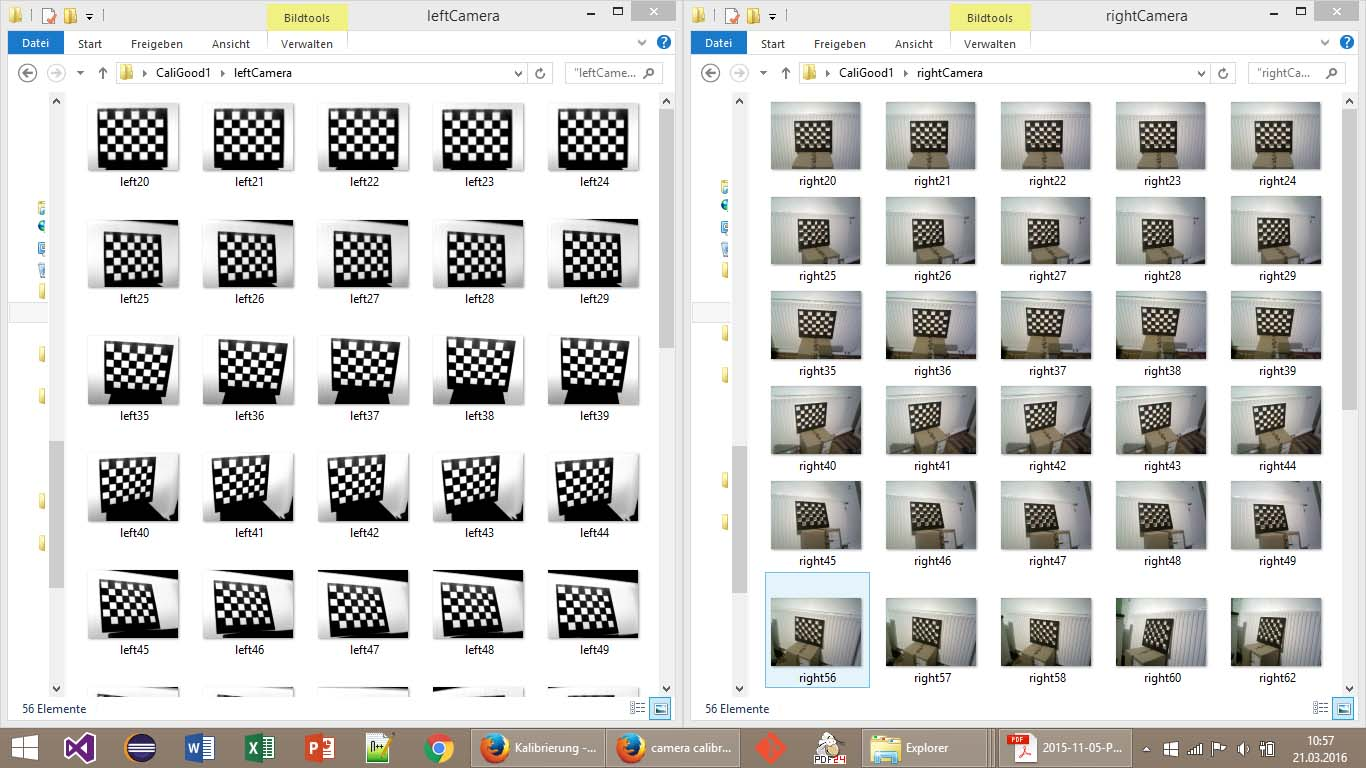
\includegraphics[width=\textwidth]{Kalibrierung/pics.jpg}}{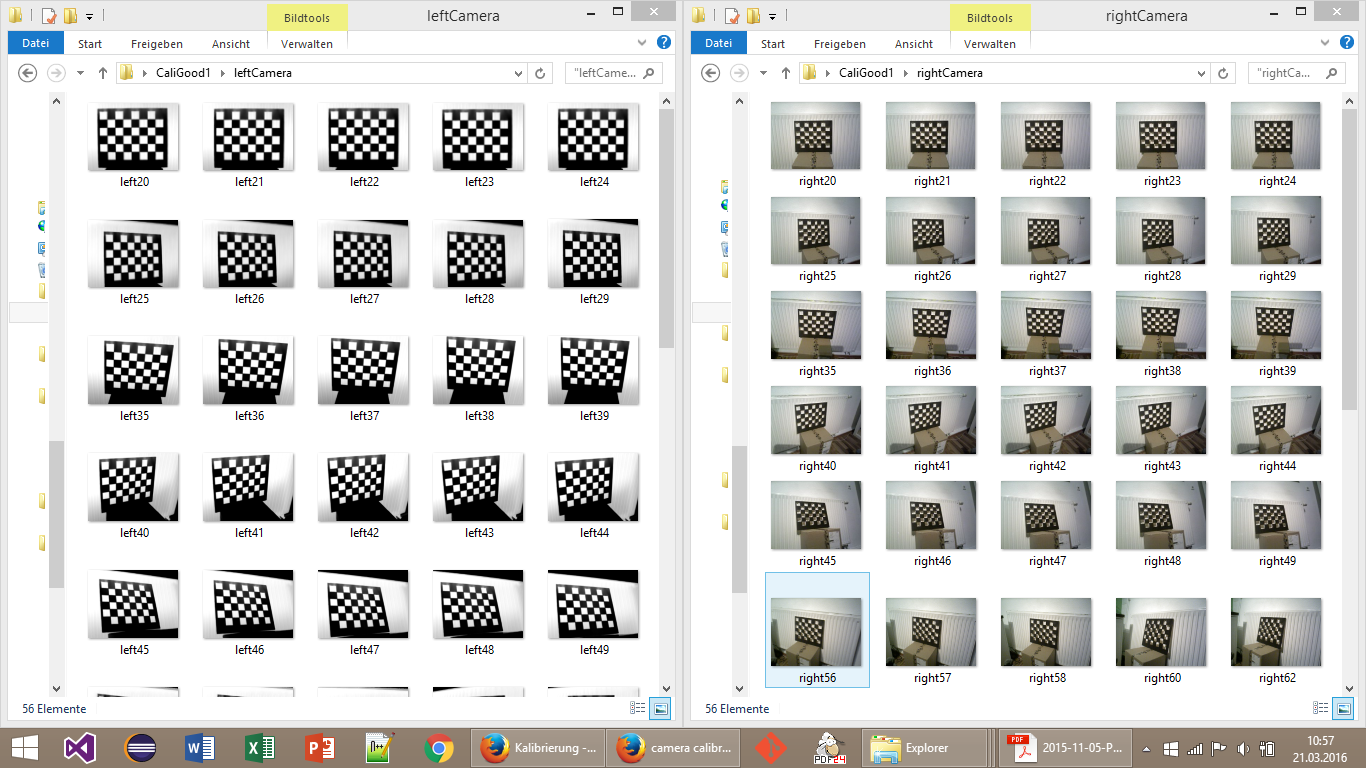
\includegraphics[width=\textwidth]{Kalibrierung/pics.png}}
	\caption{Auszug der für die Kalibrierung erstellten Bilder}
	\label{fig:calib_pics}
\end{figure}
Mithilfe der oben genannten Werten konnten wir jedes Pixel im Tiefenbild seinem zugehörigen Pixel im Wärmebild zuweisen.

\section{Kalibrierung Tiefenbild auf Wärmebild Technischer Vorgang}

\subsection{Vorgang}
\begin{enumerate}
	\item \textbf{Umwandlung Bildkoordinaten (\bzgl Tiefenbildsensor) zu Weltkoordinaten(\bzgl Tiefensensor)}
	
	Dazu wurde jedes Pixel mit den Bildkoordinaten unseres Bitmapbildes (\textbf{x},\textbf{y}) und seiner zugehörigen Distanz \textbf{z} (durch den Tiefensensor ermittelt) mithilfe der intrinsischen Kameraparameter des Tiefensensors in Weltkoordinaten(\bzgl Tiefensensor) umgewandelt.
	
	\item \textbf{Umwandlung Weltkoodinaten (\bzgl Tiefensensor) zu Weltkoordinaten (\bzgl Wärmesensor)}
	
	Diese Weltkoordinaten (\bzgl Tiefensensor) wurde dann mithilfe der extrinsischen Kameraparameter (Rotation und Translation) in die Weltkoordinaten (\bzgl Wärmesensors) umgewandelt.
	
	\item \textbf{Umwandlung Weltkoordinaten (\bzgl Wärmesensor) zu Bildkoordinaten(\bzgl Tiefenbildsensor)}
	
	Diese Weltkoordinaten (\bzgl Wärmesensor) werden dann mithilfe der intrinsischen Kameraparameter des Wärmesensors in die Bildkoordinaten (\bzgl Tiefenbildsensor) umgewandelt.
	
	Durch diese 3 Schritte können wir herausfinden, wo ein eingezeichnetes Pixel des Tiefenbildsensor sich im Bild des Wärmesensors befinden würde.
	Dadurch können wir diese Pixel dann an ihren neuen Ort verschieben.
\end{enumerate}

\subsection{Technische Details}
In unserem Projekt konnten wir die Objekte welche zwischen 1.7m und 3.7m vom Tiefenbildsensor entfernt sind genau zwischen Tiefenbildsensor und Wärmesensor kalibrieren.
Objekte zwischen 0.6m und 1.7m oder 3.7m und 8m werden, nachträglich mithilfe einer Funktion welche abhängig von der Entfernung ist, manuell nach verschoben.

Außerdem wurde bei uns bei der Berechnung der intrinsischen und extrinsischen Kameraparameter nicht Bilder des Tiefenbildsensors verwendet sondern einer RGB-Kamera welche bereits zuvor vom Hersteller aufeinander kalibriert wurde.
Grund für dies war die schlechte Erkennung des Schachbretts durch den Tiefenbildsensor.